\section{Background}\label{sec:background}

The aldermanic menu program was initiated in 1994 and continues to this day \citep{OIGaudit}. 
The program delegates approximately \$75 million every year to be split equally amongst the 50 aldermen in Chicago's city council to be spent on projects they unilaterally select for their ward, given a ``menu'' of acceptable expenditures. 
Each alderman allocates approximately \$1.5 million per year to their ward.
Chicago's Office of Budget and Management (OBM) tracks the spending and its Department of Transportation (CDOT) manages the program.
Each ward is defined to be approximately equal by population every 10 years, depending on the decennial census results, but the overall map is subject to a city council vote for approval.
The Chicago Board of Elections draws the precinct map using the ward map, according to the available number of polling places, and each contain between 500 to 800 voters \citep{Crowley_2022}.
The 2012-2023 ward map (which has the majority of the data used in this paper) contains 2069 precints for the 50 wards, averaging 41.38 precincts per ward \citep{Crowley_2022}.
Each year in the spring, the Mayor, CDOT, and OBM send letters to the aldermen explaining the program and providing a menu of cost estimates and a list of possible projects.
Before the aldermen select projects, CDOT and OBM provide a briefing packet with 311 complaint data.
Finally, aldermen more or less spend the money as they see fit, with the only hard restriction being that they cannot spend more than \$1.32 million on any one project.
Because this program and elections occur in the spring, new aldermen can only spend their entire menu funds the following year and often rely on the previous Alderman's programmed budget the year they are elected.

``Off-menu'' expenditures are also allowed, of which most ``off-menu'' funds go towards Parks, Chicago Public Schools, and miscellaneous beautification projects such as trees, murals, decorative garbage cans, designer bike racks, and more \citep{OIGaudit}. 
While on-menu items are typically also provided by other funding sources within Chicago's Capital Improvement Program, off-menu items such as murals and statues are usually directly credited to the aldermen, thus giving an incentive to reward supporters' loyalty with public goods.
The program is unique insofar as it gives elected politicians a wide berth over a significant portion of the City's infrastructure budget and allows its use for items one does not typically think of as core infrastructure. 
An example of a portion of a menu from 2013 is shown below in Figure~\ref{fig:menu_example}.


\begin{figure}[H]
    \centering
    \caption{An Example of a menu from 2012/2013}\label{fig:menu_example}
    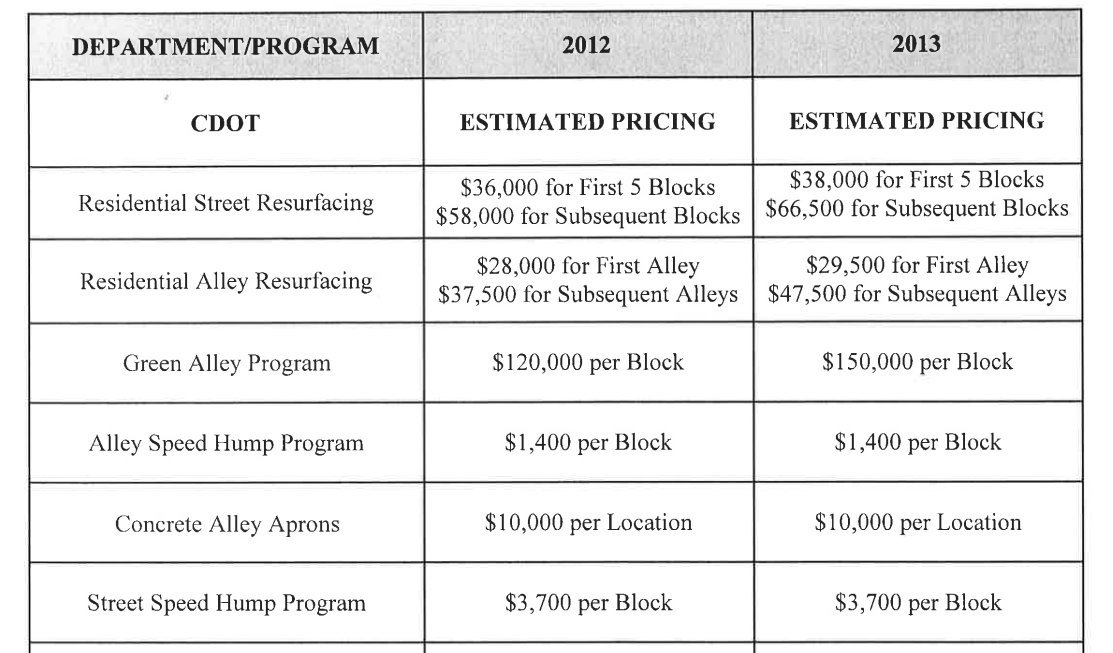
\includegraphics[scale=0.38]{input/menu_example.png}
\end{figure}

The Chicago Office of the Inspector General audited the program in 2017 and found that the program was rife with misallocation -- because wards are defined to be approximately equal by population but not equal by infrastructure needs, so some dense wards get 80\% or more of their needs met while others get only 10\% or less \citep{OIGaudit}.


Thus, the OIG found that the program resulted in significant funding disparities between wards relative to infrastructure needs.
Secondly, the OIG audit found that from 2012 through 2015, the program permitted aldermen to use \$ 15.1 million in menu funds for projects unrelated to so-called ``core'' infrastructure.
Finally, the OIG audit found that CDOT allowed aldermen to use \$825,292 of menu funds on projects outside of the ward they were elected to represent so that they could spend it on the wards they were running for reelection in.
